\chap{LED Animations}

\section{Introduction}
In this manual, the STM32CubeIDE is used as an editor to program the ARM micro-controller. STM32CubeIDE is an advanced C/C++ development platform with peripheral configuration, code generation, code compilation, and debug features for STM32 microcontrollers and microprocessors.\\

\begin{figure}[!htp]
    \centering
    
\includegraphics[width=4in]{source/picture/bai_1/cubeide.jpg}
    \caption{\textit{STM32Cube IDE for STM32 Programming}}
    \label{bai1_cube}
\end{figure}

The most interest of STM32CubeIDE is that after the selection of an empty STM32 MCU or MPU, or preconfigured microcontroller or microprocessor from the selection of a board, the initialization code generated automatically. At any time during the development, the user can return to the initialization and configuration of the peripherals or middleware and regenerate the initialization code with no impact on the user code. This feature can simplify the initialization process and speedup the development application running on STM32 micro-controller. The software can be downloaded from the link bellow:
\begin{center}
    \link{https://ubc.sgp1.digitaloceanspaces.com/BKU\_Softwares/STM32/stm32cubeide\_1.7.0.zip}
\end{center}

Moreover, for a hangout class, the program is firstly simulated on Proteus. Students are also supposed to download and install this software as well:

\begin{center}
    \link{https://ubc.sgp1.digitaloceanspaces.com/BKU\_Softwares/STM32/Proteus\_8.10\_SP0\_Pro.exe}
\end{center}

The rest of this manual consists of:
\begin{itemize}
    \item Create a project on STM32Cube IDE
    \item Create a project on Proteus
    \item Simulate the project on Proteus
\end{itemize}

Finally, students are supposed to finish 10 different projects. 

\newpage
\section{First project on STM32Cube}
\textbf{Step 1: } Launch STM32CubeIDE, from the menu \textbf{File}, select \textbf{New}, then chose \textbf{STM32 Project} 

\begin{figure}[!htp]
    \centering
    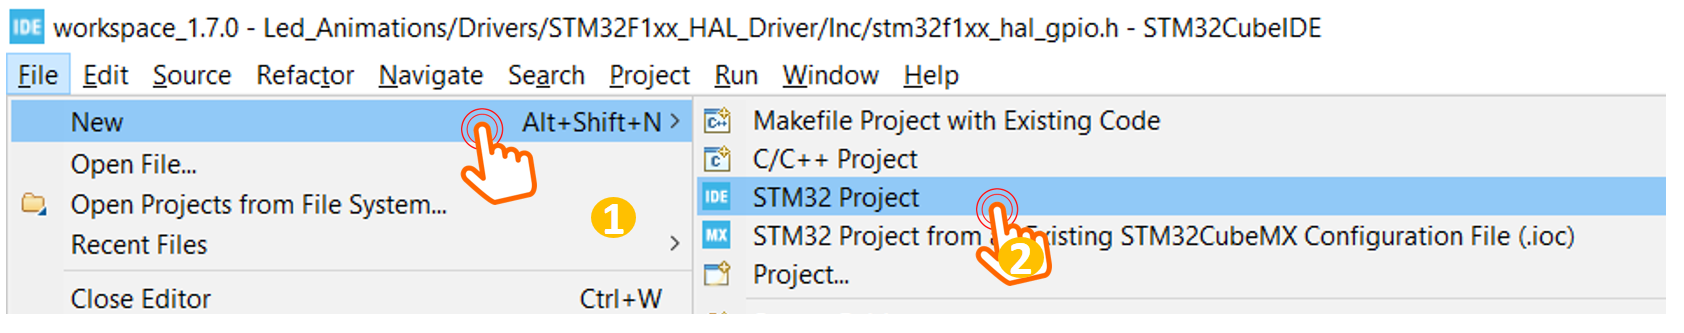
\includegraphics[width=5in]{source/picture/bai_1/stm_01.PNG}
    \caption{\textit{Create a new project on STM32CubeIDE}}
    \label{bai1_stm1}
\end{figure}

The IDE needs to download some packages, which normally takes time in this first time a project is created.\\

\textbf{Step 2: } Select the STM32F103C6 in the following dialog, then click on \textbf{Next}

\begin{figure}[!htp]
    \centering
    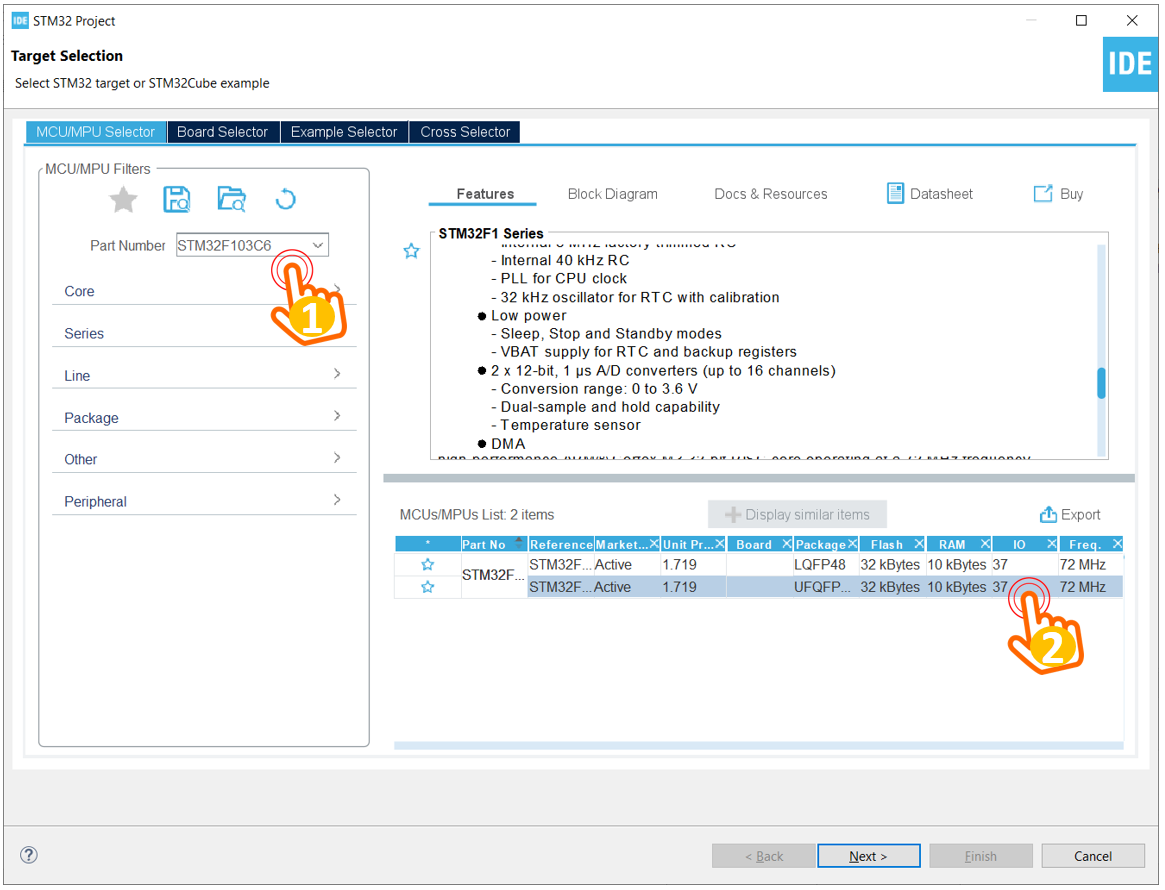
\includegraphics[width=5in]{source/picture/bai_1/stm_02.PNG}
    \caption{\textit{Select the target device}}
    \label{bai1_stm2}
\end{figure}

\textbf{Step 3: } Provide the \textbf{Name} and the \textbf{Location} for the project.

\newpage
\begin{figure}[!htp]
    \centering
    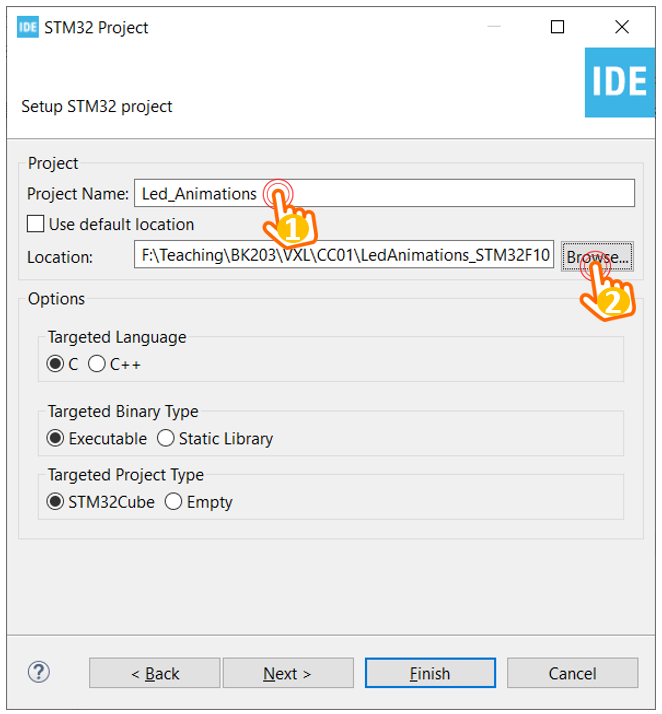
\includegraphics[width=3.5in]{source/picture/bai_1/stm_03.PNG}
    \caption{\textit{Select the target device}}
    \label{bai1_stm3}
\end{figure}

It is important to notice that the \textbf{Targeted Project Type} should be \textbf{STM32Cube}. In the case this option is disable, step 1 must be repeated. The location path should not contain special characters (e.g. the space). Finally, click on the \textbf{Next} button.\\

\textbf{Step 4: } On the last dialog, just keep the default firmware version and click on \textbf{Finish} button.

\begin{figure}[!htp]
    \centering
    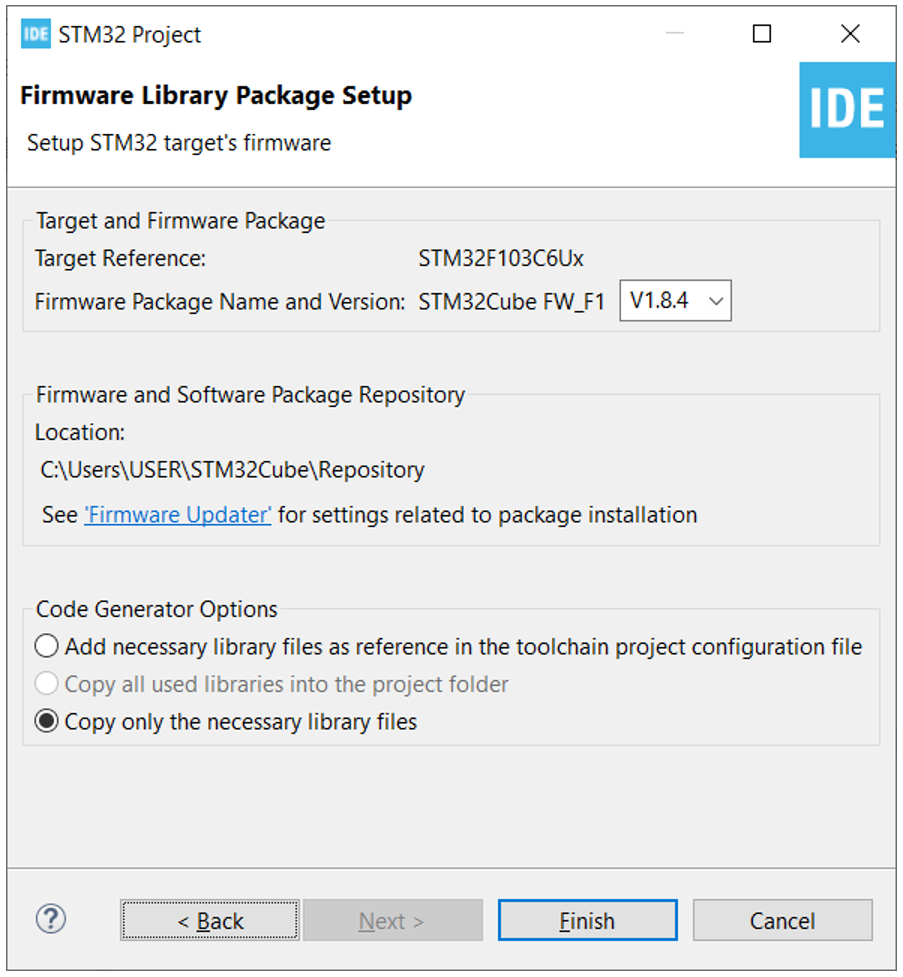
\includegraphics[width=3.5in]{source/picture/bai_1/stm_04.PNG}
    \caption{\textit{Keep default firmware version}}
    \label{bai1_stm4}
\end{figure}

\textbf{Step 5: } The project is created and the wizard for configuration is display. This utility from CubeIDE can simplify the configuration process for an ARM micro-controller like the STM32.

\begin{figure}[!htp]
    \centering
    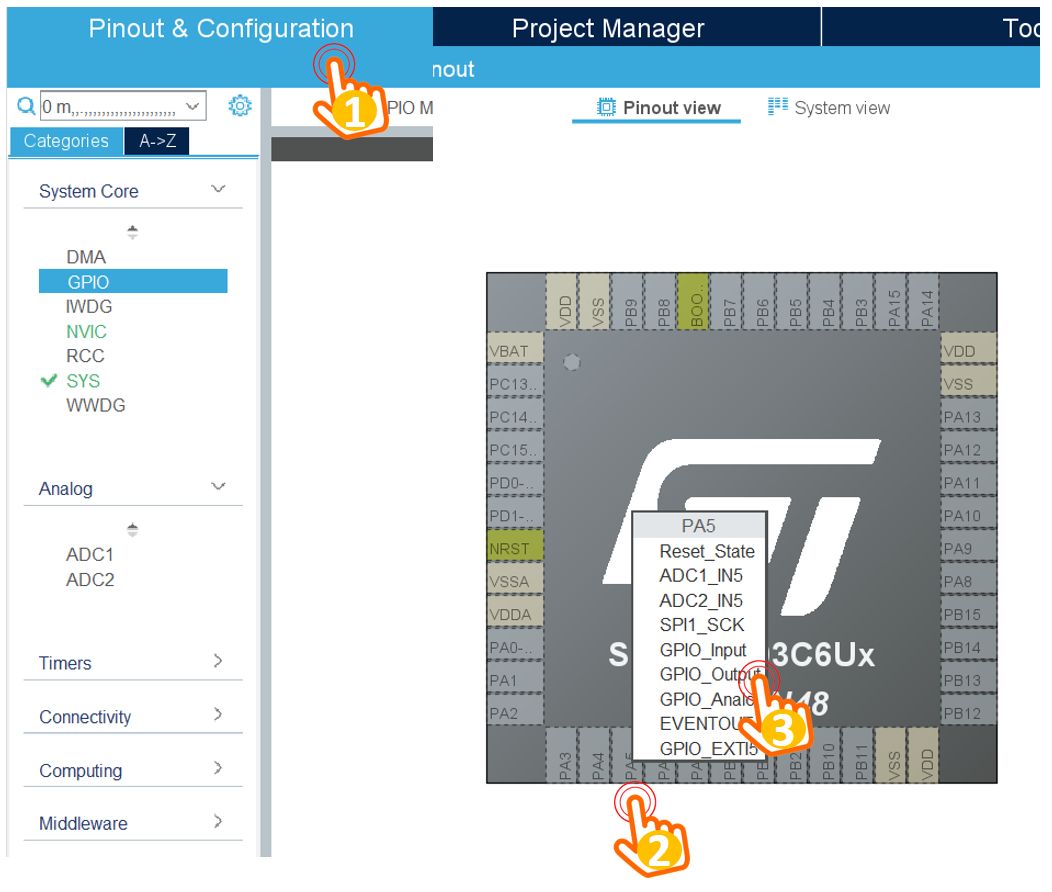
\includegraphics[width=3.5in]{source/picture/bai_1/stm_05.PNG}
    \caption{\textit{Set PA5 to GPIO Output mode}}
    \label{bai1_stm5}
\end{figure}

From the configuration windows, select \textbf{Pin configuration}, select the pin \textbf{PA5} and set to \textbf{GPIO Output} mode, since this pin is connected to an LED in the STM32 development kit.\\

\textbf{Step 6: } Right click on PA5 and select \textbf{Enter user lable}, and provide the name for this pin (e.g. \textbf{LED\_RED}). This step helps programming afterward more memorable.

\begin{figure}[!htp]
    \centering
    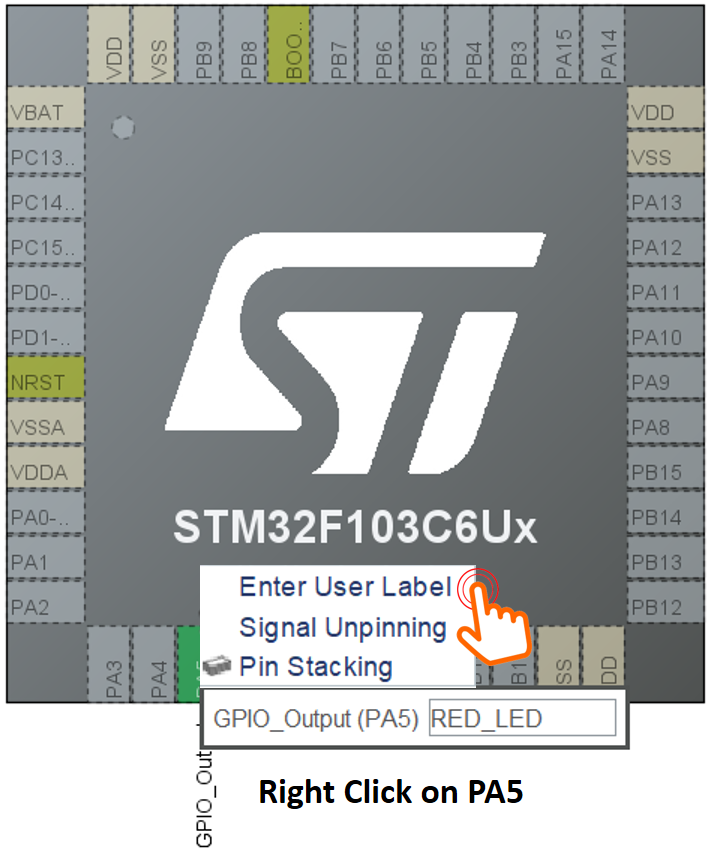
\includegraphics[width=2.5in]{source/picture/bai_1/stm_06.PNG}
    \caption{\textit{Provide a name for PA5}}
    \label{bai1_stm6}
\end{figure}

Finally, save the configuration process by pressing \textbf{Ctrl + S} and confirm this step by clicking on \textbf{OK} button. The code generation is started.\\

\textbf{Step 7: } Implement the first blinky project in the main function as follow:
\begin{lstlisting}[caption=First blinky LED project]
int main(void)
{
  /* USER CODE BEGIN 1 */

  /* USER CODE END 1 */

  /* MCU Configuration--------------------------------------------------------*/

  /* Reset of all peripherals, Initializes the Flash interface and the Systick. */
  HAL_Init();

  /* USER CODE BEGIN Init */

  /* USER CODE END Init */

  /* Configure the system clock */
  SystemClock_Config();

  /* USER CODE BEGIN SysInit */

  /* USER CODE END SysInit */

  /* Initialize all configured peripherals */
  MX_GPIO_Init();
  /* USER CODE BEGIN 2 */

  /* USER CODE END 2 */

  /* Infinite loop */
  /* USER CODE BEGIN WHILE */
 
  while (1)
  {
	  HAL_GPIO_TogglePin(LED_RED_GPIO_Port, LED_RED_Pin);
	  HAL_Delay(1000);
    /* USER CODE END WHILE */

    /* USER CODE BEGIN 3 */
  }
  /* USER CODE END 3 */
}
\end{lstlisting}

Actually, what is added to the main function is line number 34 and 35. Please put your code in a right place, otherwise it can be deleted when the code is generated (e.g. change the configuration of the project). When coding, frequently use the suggestions by pressing \textbf{Ctrl+Space}.

\textbf{Step 7: } Due to the simulation on Proteus, the hex file should be generated from STM32Cube IDE. From menu \textbf{Project}, select \textbf{Properties} to open the dialog bellow:

\begin{figure}[!htp]
    \centering
    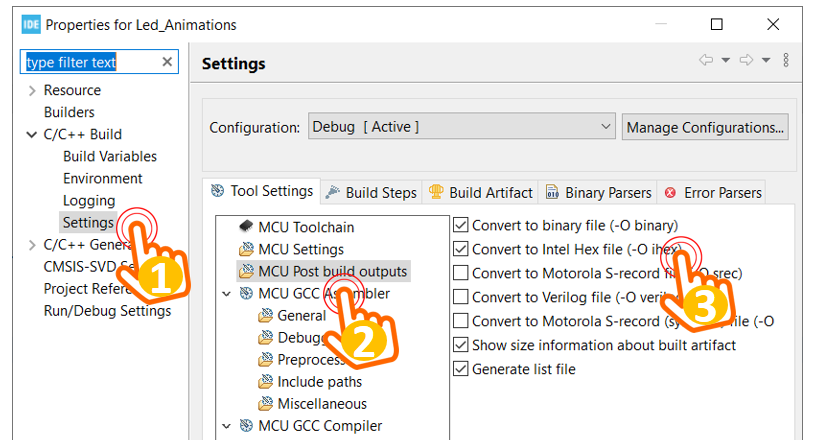
\includegraphics[width=5in]{source/picture/bai_1/stm_07.PNG}
    \caption{\textit{Config for hex file output}}
    \label{bai1_pic5}
\end{figure}

Navigate to \textbf{C/C++ Build}, select \textbf{Settings, MCU Post build outputs}, and check to the \textbf{Intel Hex file}. \\

\textbf{Step 8: } Build the project by clicking on menu \textbf{Project} and select \textbf{Build Project}. Please check on the output console of the IDE to be sure that the hex file is generated, as follow:

\begin{figure}[!htp]
    \centering
    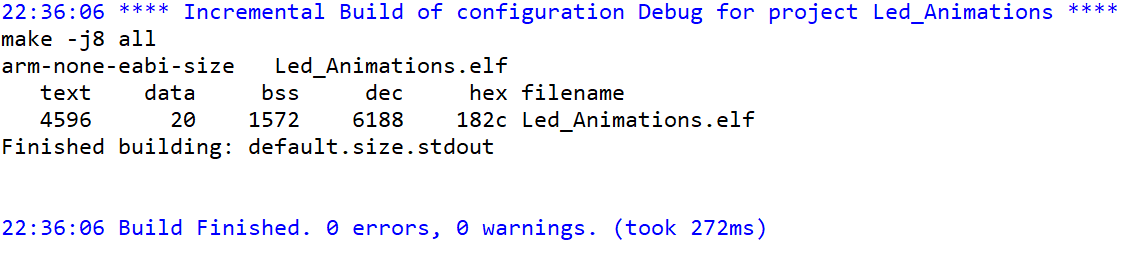
\includegraphics[width=5in]{source/picture/bai_1/stm_08.PNG}
    \caption{\textit{Compile the project and generate Hex file}}
    \label{bai1_pic8}
\end{figure}

The hex file is located under the \textbf{Debug} folder of your project, which is used for the simulation in Proteus afterward. In the case a development kit is connected to your PC, from menu \textbf{Run}, select \textbf{Run} to download the program to the hardware platform. \\

In the case there are multiple project in a work-space, double click on the project name to activate this project. Whenever a project is built, check the output files to make sure that you are working in a right project.


\newpage
\section{Simulation on Proteus}
For an online training, a simulation on Proteus can be used. The details to create an STM32 project on Proteus are described bellow.\\

\textbf{Step 1: } Launch Proteus (\textbf{with administration access}) and from menu \textbf{File}, select \textbf{New Project}.\\

\begin{figure}[!htp]
    \centering
    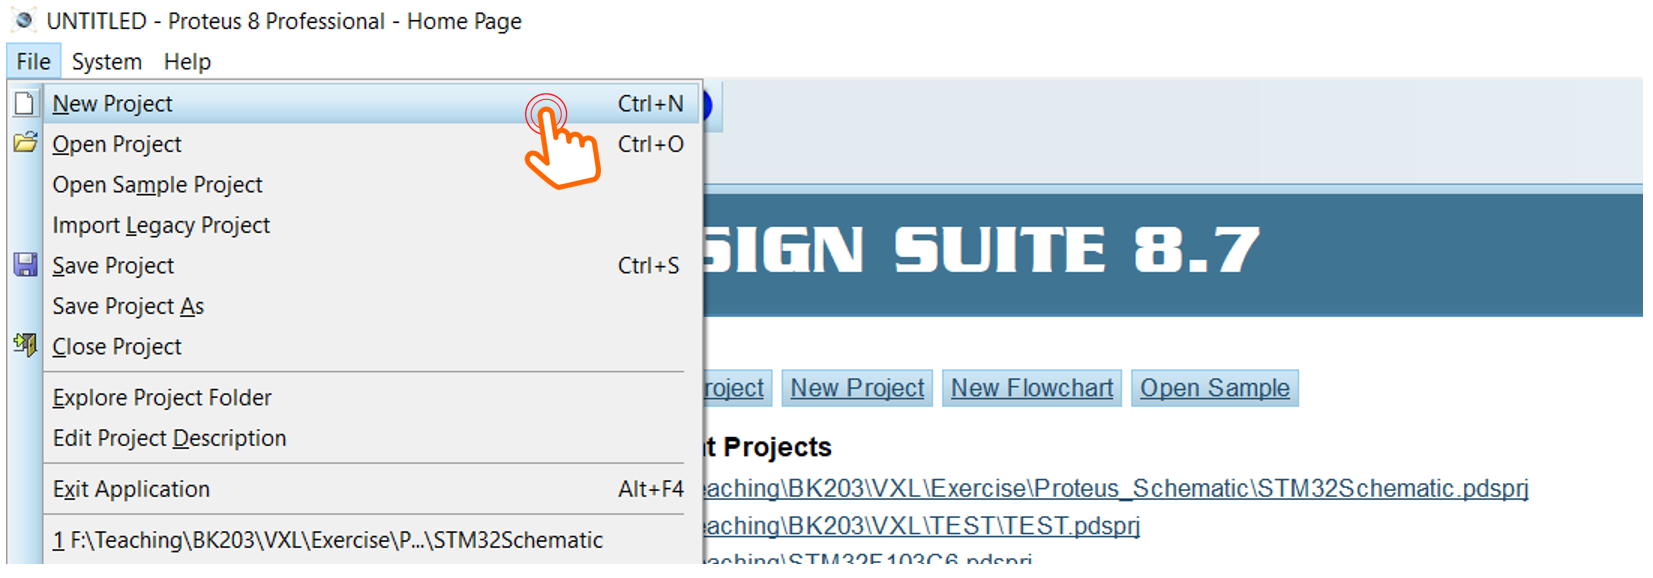
\includegraphics[width=5in]{source/picture/bai_1/pic5.PNG}
    \caption{\textit{Create a new project on Proteus}}
    \label{bai1_pic5}
\end{figure}


\textbf{Step 2: } Provide the name and the location of the project, then click on \textbf{Next} button.\\

\begin{figure}[!htp]
    \centering
    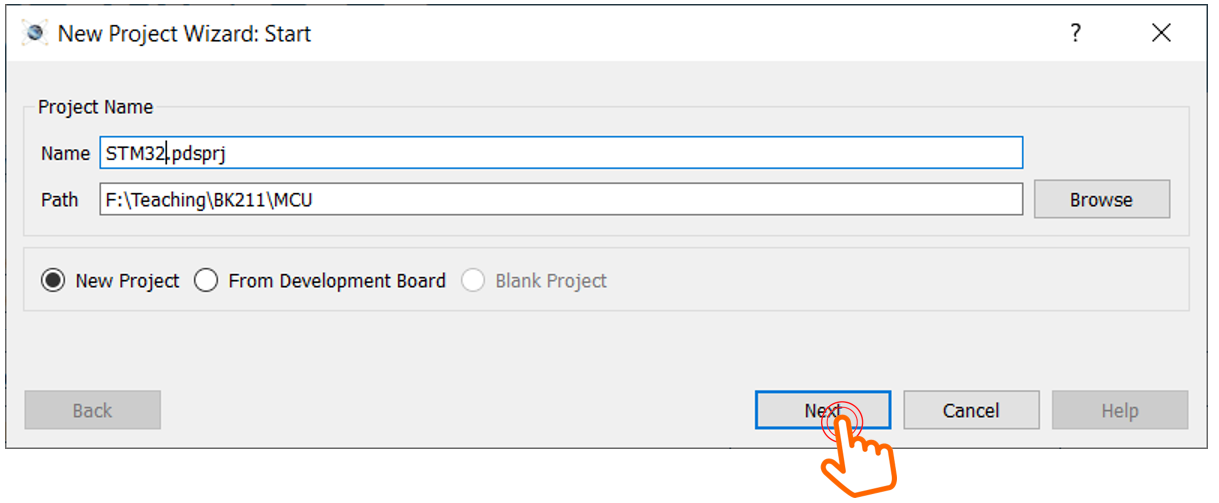
\includegraphics[width=4in]{source/picture/bai_1/pic6.PNG}
    \caption{\textit{Provide project name and location}}
    \label{bai1_pic6}
\end{figure}

\textbf{Step 3: } For following dialog, just click on \textbf{Next} button as just a schematic is required for the lab.

\begin{figure}[!htp]
    \centering
    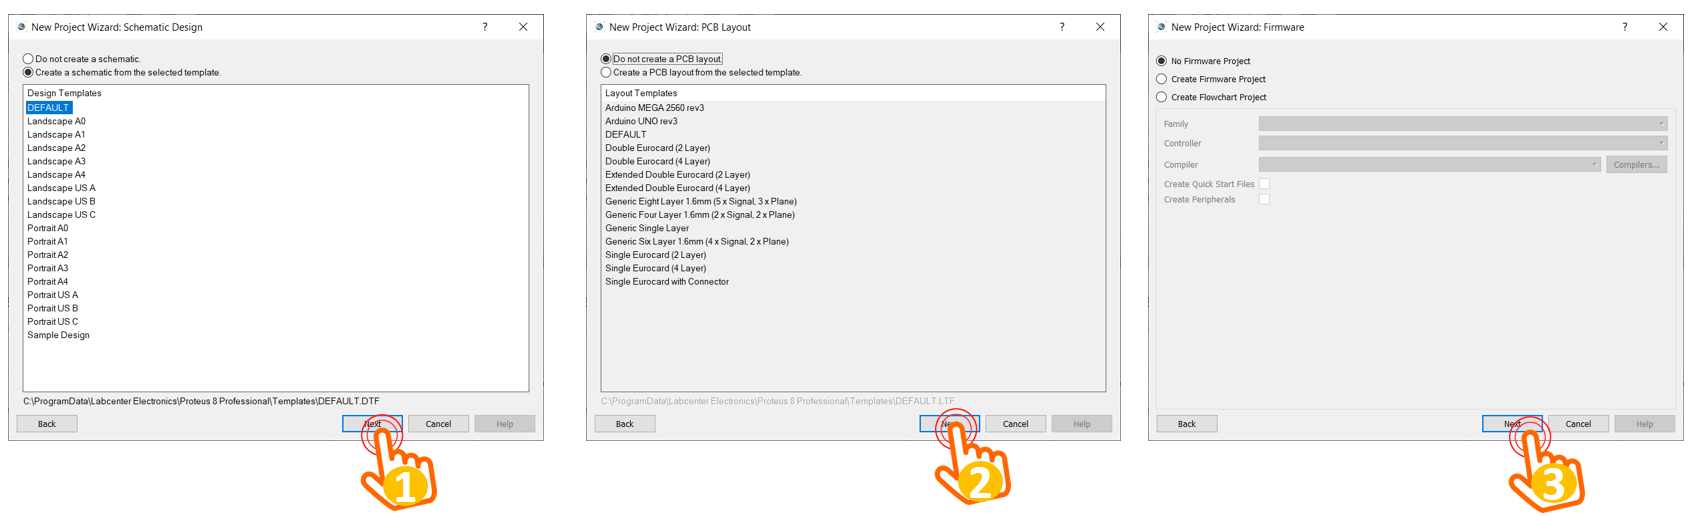
\includegraphics[width=5.5in]{source/picture/bai_1/pic7.PNG}
    \caption{\textit{Keep the default options by clicking on Next}}
    \label{bai1_pic7}
\end{figure}
\newpage
\textbf{Step 4: } Finally, click on \textbf{Finish} button to close the project wizard. \\

\begin{figure}[!htp]
    \centering
    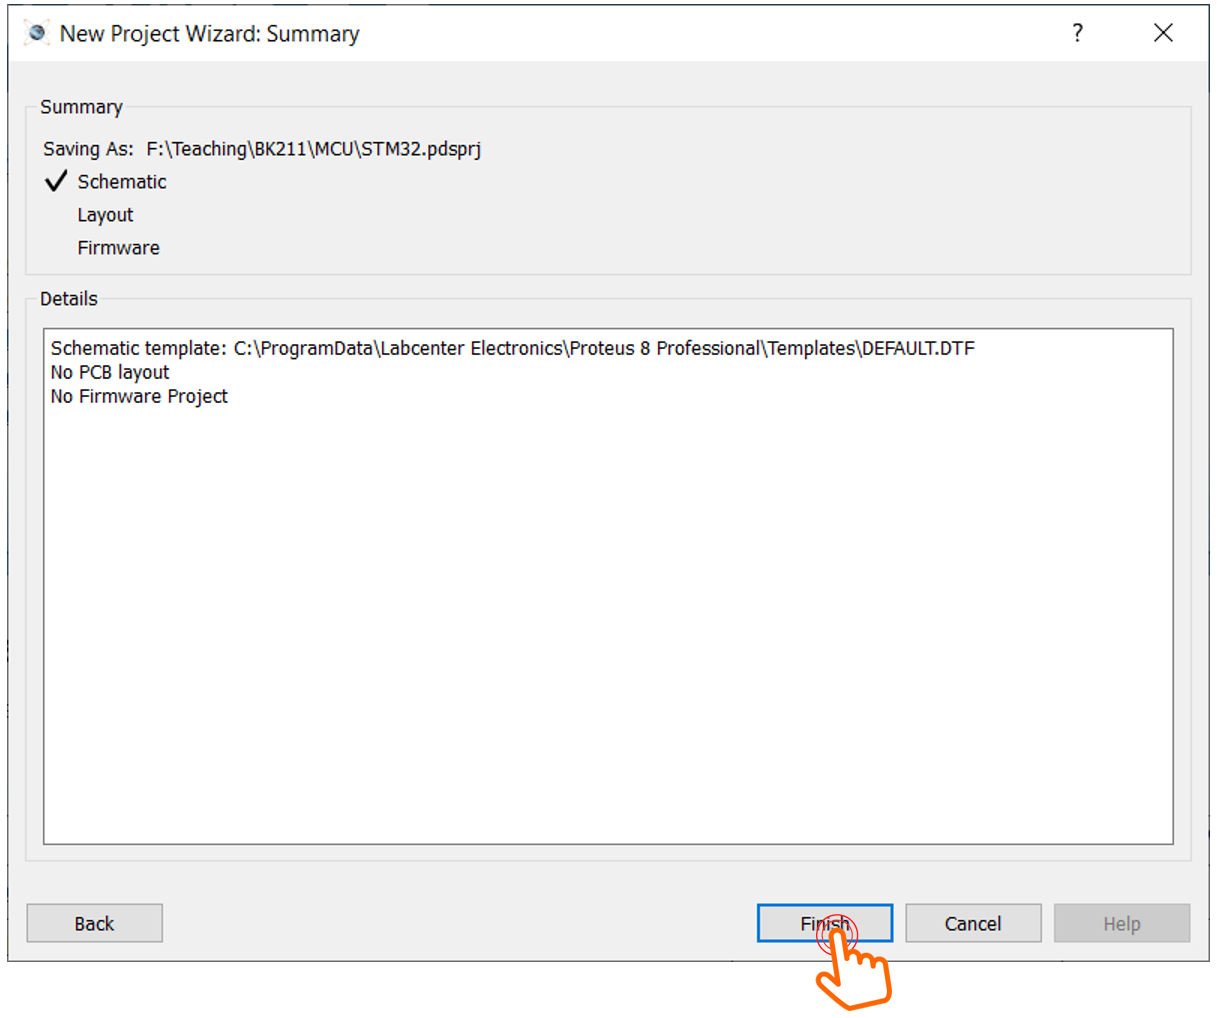
\includegraphics[width=4in]{source/picture/bai_1/pic8.PNG}
    \caption{\textit{Finish the project wizard}}
    \label{bai1_pic8}
\end{figure}

\textbf{Step 5: } On the main page of the project, right click to select \textbf{Place, Components, From Libraries}, as follows:
\begin{figure}[!htp]
    \centering
    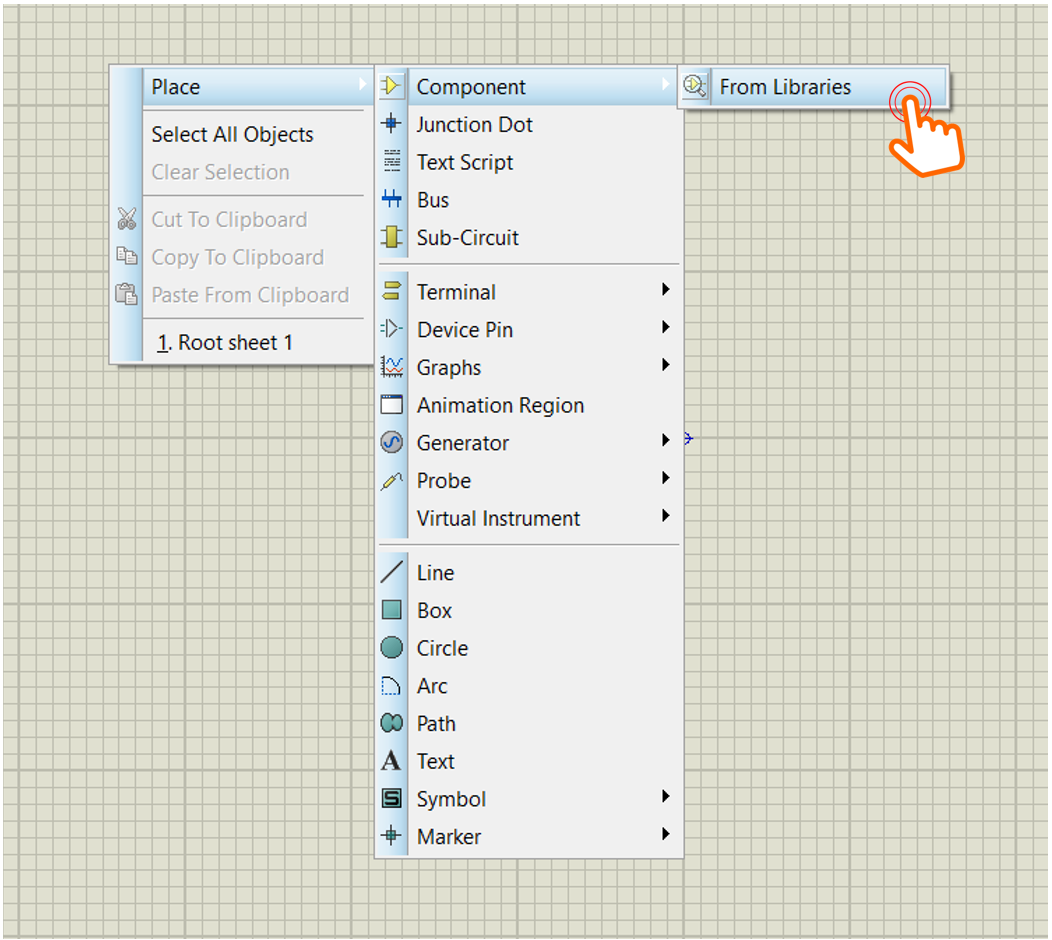
\includegraphics[width=4in]{source/picture/bai_1/pic9.PNG}
    \caption{\textit{Select a component from the library}}
    \label{bai1_pic9}
\end{figure}

\textbf{If there is an error with no library found, please restart the Proteus software with Run as administrator option.\\}

\textbf{Step 6: } From the list of components in the library, select STM32F103C6, as follows:

\begin{figure}[!htp]
    \centering
    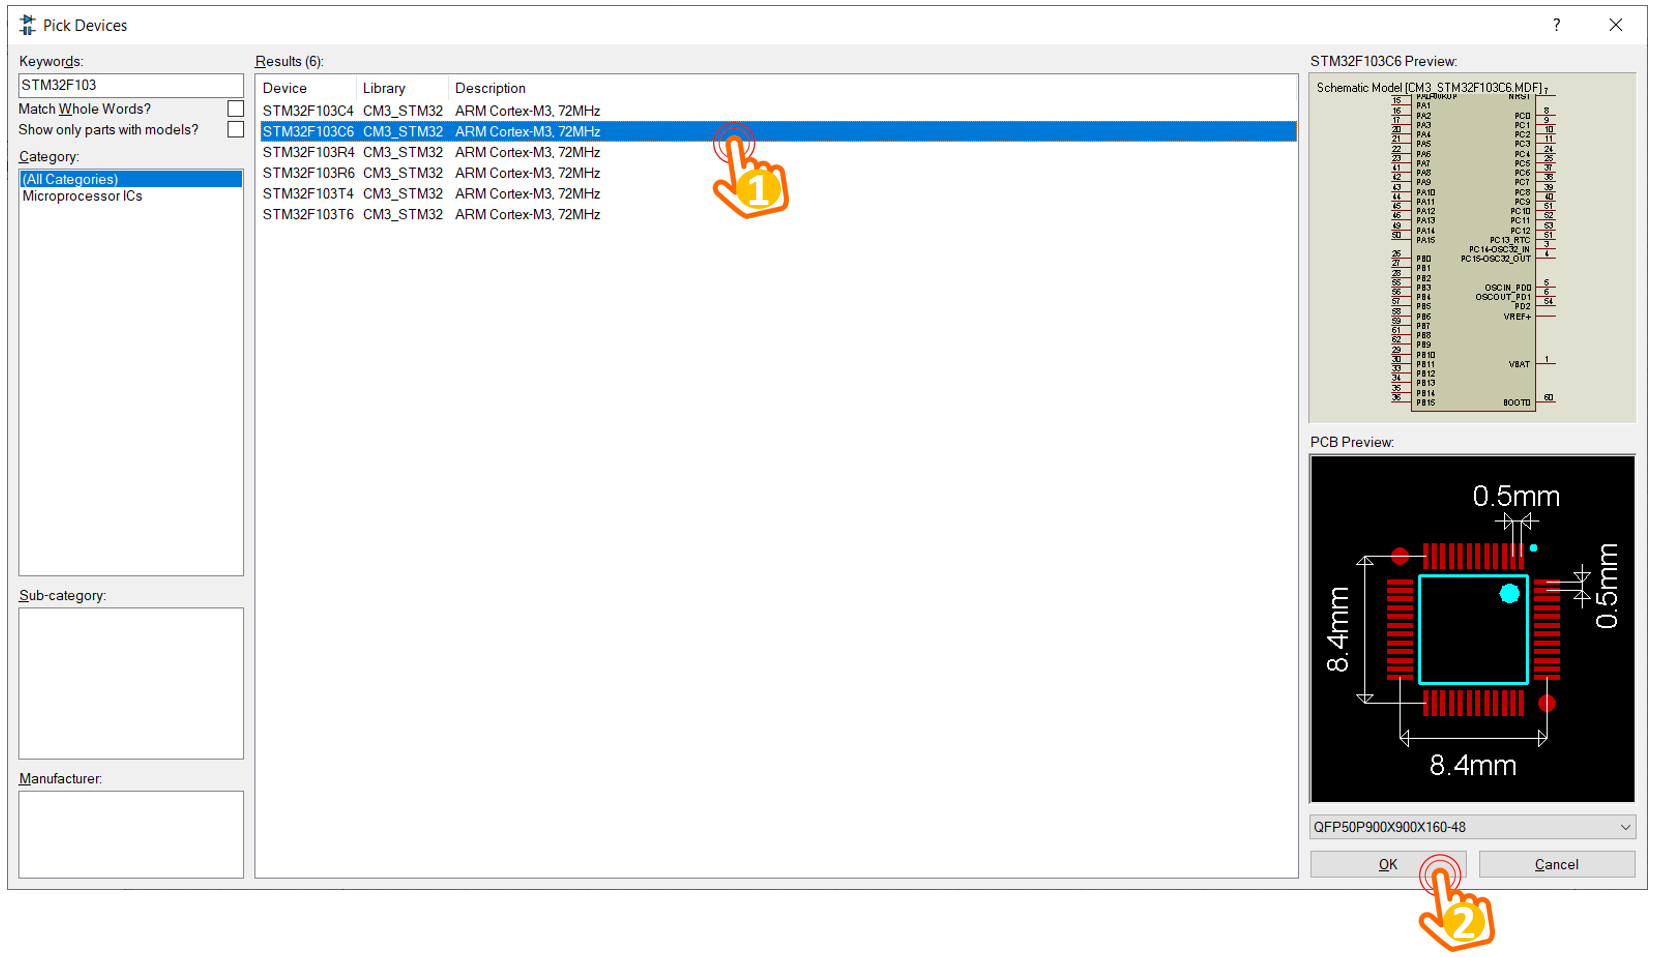
\includegraphics[width=5.5in]{source/picture/bai_1/pic10.PNG}
    \caption{\textit{Select STM32F103C6}}
    \label{bai1_pic10}
\end{figure}

Repeat step 5 and 6 to select an LED, named \textbf{LED-RED} in Proteus. Finally, these components are appeared on the DEVICES windows, which is on left hand side as follows:
\begin{figure}[!htp]
    \centering
    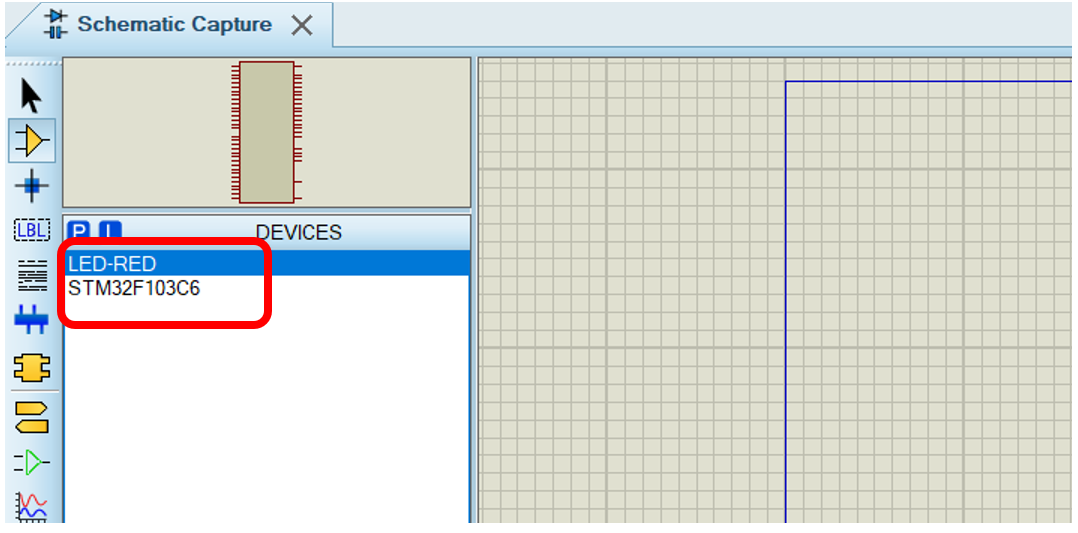
\includegraphics[width=4in]{source/picture/bai_1/pic11.PNG}
    \caption{\textit{STM32 and an LED in the project}}
    \label{bai1_pic9}
\end{figure}

\textbf{Step 7: } Place the components to the project: right click on the main page, select on \textbf{Place, Component}, and select device added in Step 6. To add the Power and the Ground,  right click on the main page, select on \textbf{Place, Terminal}. The result in this step is expected as follows:
\newpage
\begin{figure}[!htp]
    \centering
    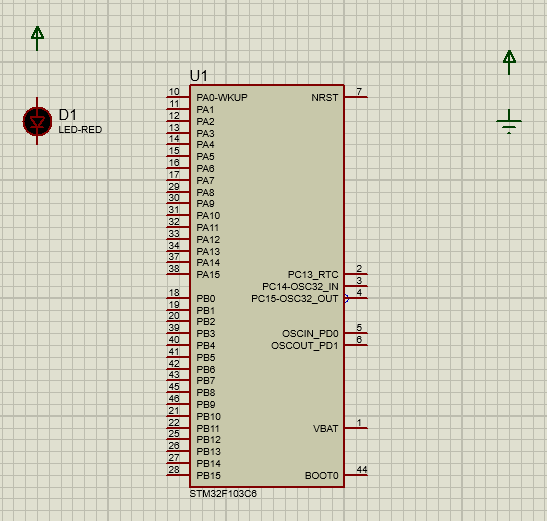
\includegraphics[width=4in]{source/picture/bai_1/pic14.PNG}
    \caption{\textit{Place components to the project}}
    \label{bai1_pic14}
\end{figure}

\textbf{Step 8: } Start wiring the circuit. The negative pin of the LED is connected to PA5 while its positive pin is connected to the power supply. For the power and the ground on the right, just make a short wire, which will labeled in the next step.

\begin{figure}[!htp]
    \centering
    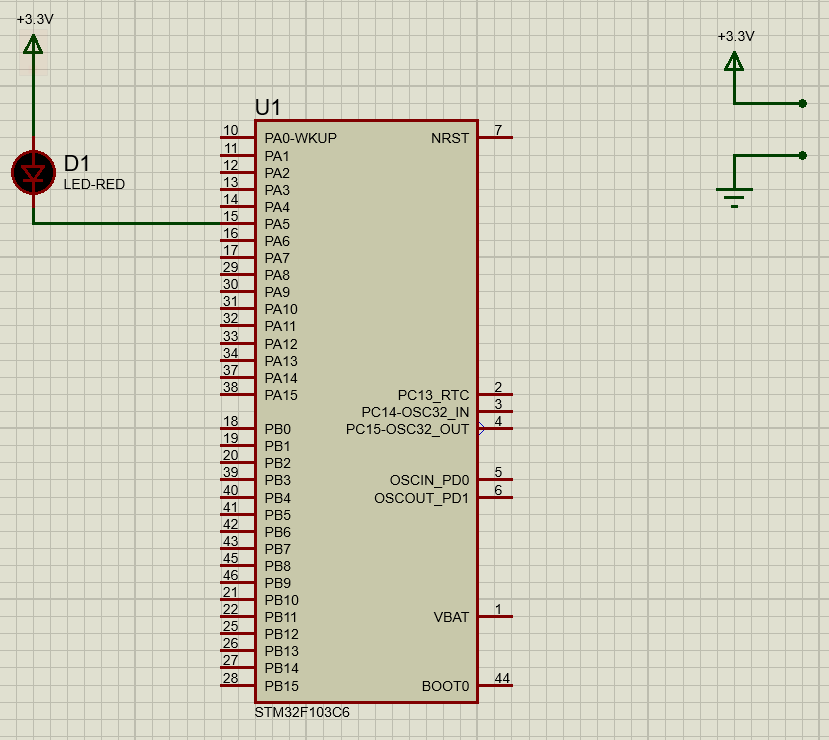
\includegraphics[width=4in]{source/picture/bai_1/pic15.PNG}
    \caption{\textit{Connect components and set the power to 3.3V}}
    \label{bai1_pic15}
\end{figure}

In this step, also double click on the power supply in order to provide the String property to \textbf{+3.3V}.

\textbf{Step 8: } Right click on the wire of the power supply and the ground, and select \textbf{Place wire Label}

\begin{figure}[!htp]
    \centering
    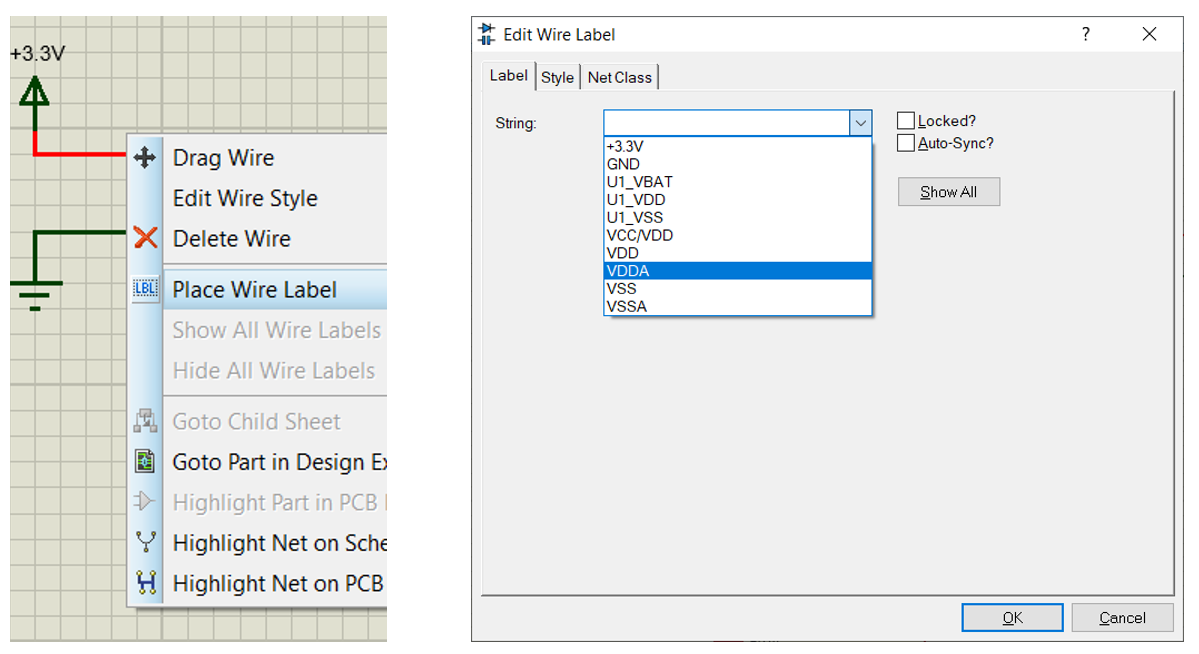
\includegraphics[width=4in]{source/picture/bai_1/pic16.PNG}
    \caption{\textit{Place label for Power and Ground}}
    \label{bai1_pic16}
\end{figure}

This step is required as VDDA and VSSA of the STM32 must be connected to provide the reference voltage. Therefore, VDDA is connected to 3.3V, while the VSSA is connected to the Ground. Finally, the image of our schematic is shown bellow:

\begin{figure}[!htp]
    \centering
    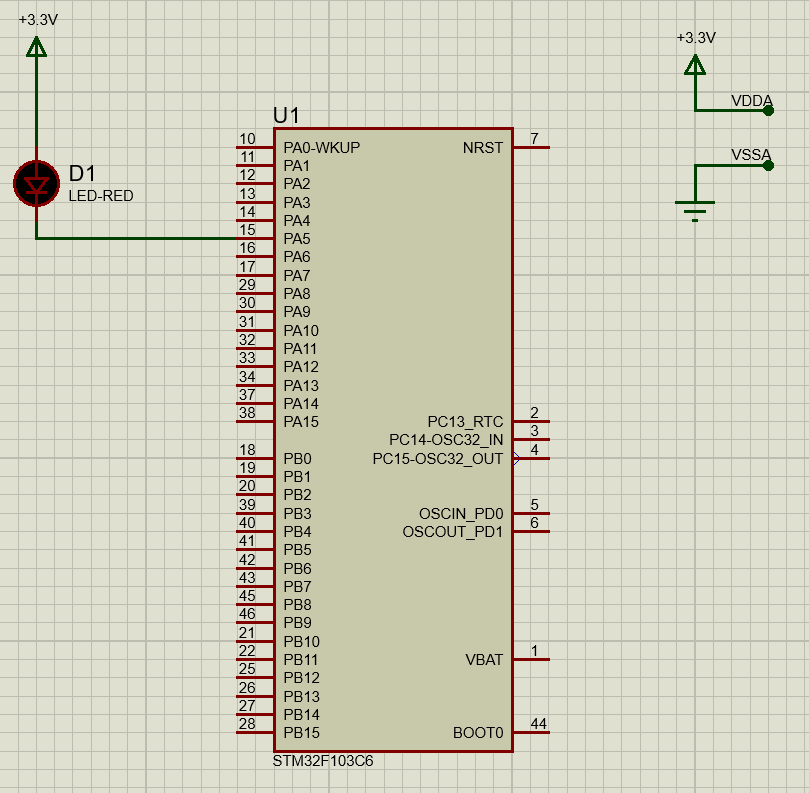
\includegraphics[width=4in]{source/picture/bai_1/pic17.PNG}
    \caption{\textit{Finalize the schematic}}
    \label{bai1_pic17}
\end{figure}
\newpage
\textbf{Step 9: } Double click on the STM32, and set the \textbf{Program File} to the Hex file, which is generated from Cube IDE, as following:

\begin{figure}[!htp]
    \centering
    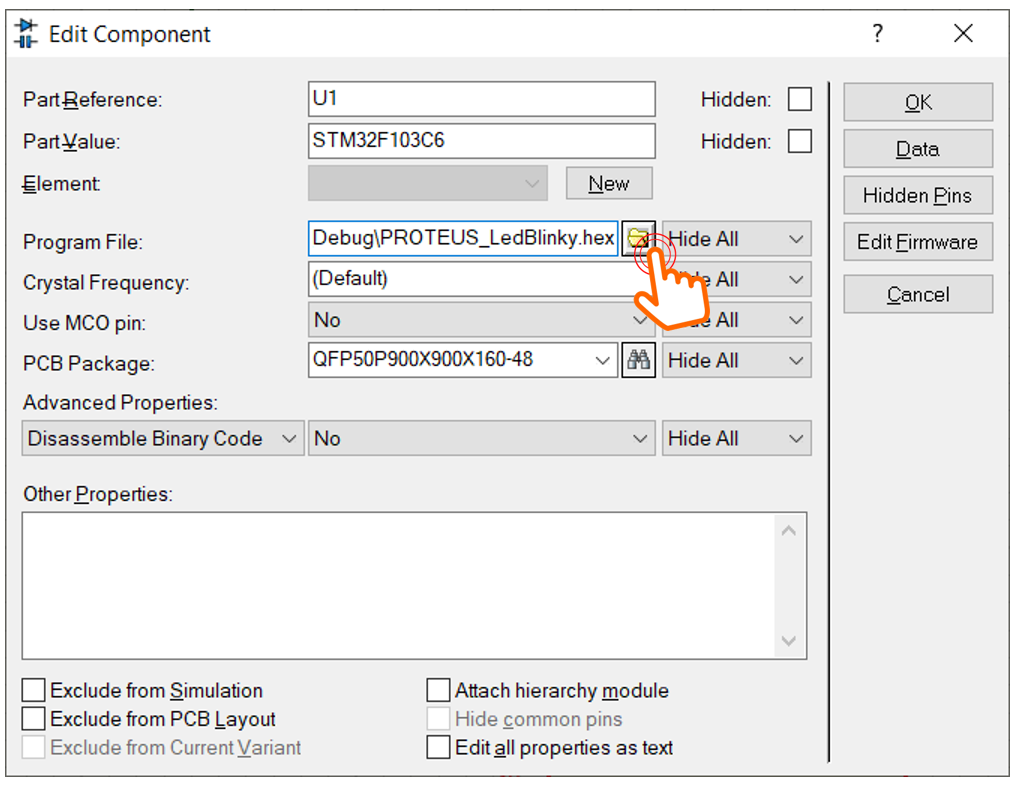
\includegraphics[width=4in]{source/picture/bai_1/pic18.PNG}
    \caption{\textit{Set the program of the STM32 to the hex file from Cube IDE}}
    \label{bai1_pic18}
\end{figure}

From now, the simulation is ready to start by clicking on the menu \textbf{Debug}, and select on \textbf{Run simulation}. To stop the simulation, click on \textbf{Debug} and select \textbf{Stop VMS Debugging}. Moreover, there are some quick access bottom on the left corner of the Proteus to start or stop the simulation, as shown following:\\
\begin{figure}[!htp]
    \centering
    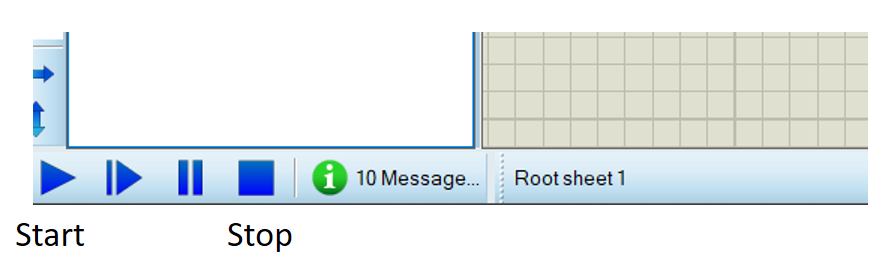
\includegraphics[width=4in]{source/picture/bai_1/pic18a.PNG}
    \caption{\textit{Quick access buttons to start and stop the simulation}}
    \label{bai1_pic18}
\end{figure}

If everything is success, students can see the LED is blinking every second. Please stop the simulation before updating the project, either in Proteus or STM32Cube IDE. However, the step 9 (set the program file for STM32 in Proteus) is required to do once. Beside the toggle instruction, student can set or reset a pin as following:

\begin{lstlisting}[caption=An example for LED blinky]
while (1){
  HAL_GPIO_WritePin(LED_RED_GPIO_Port, LED_RED_Pin, GPIO_PIN_SET);
  HAL_Delay(1000);
  HAL_GPIO_WritePin(LED_RED_GPIO_Port, LED_RED_Pin, GPIO_PIN_RESET);
  HAL_Delay(1000);
}
\end{lstlisting}
\newpage
\section{Exercise and Report}
\subsection{Exercise 1}
From the simulation on Proteus, one more LED is connected to pin \textbf{PA6} of the STM32 (negative pin of the LED is connected to PA6). The component suggested in this exercise is \textbf{LED-YELLOW}, which can be found from the device list.\\



In this exercise, the status of two LEDs are switched every 2 seconds, as demonstrated in the figure bellow.

\begin{figure}[!htp]
    \centering
    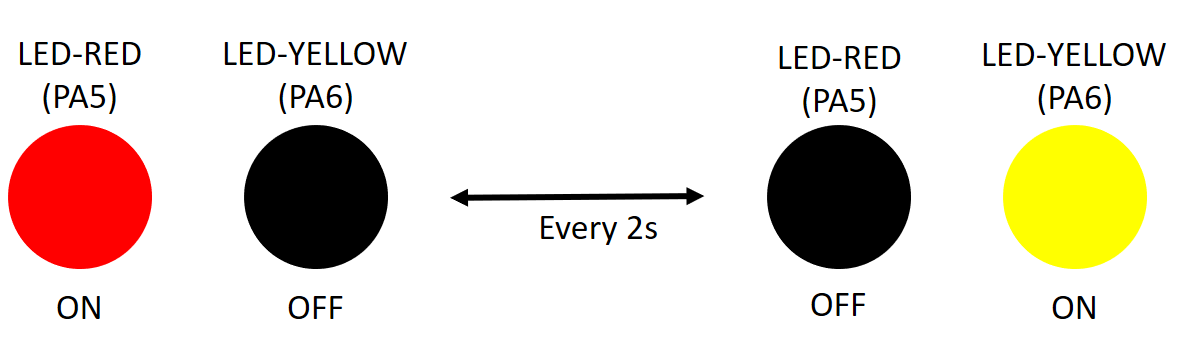
\includegraphics[width=5in]{source/picture/bai_1/pic1.PNG}
    \caption{\textit{State transitions for 2 LEDs}}
    \label{bai1_pic1}
\end{figure}

\textbf{Report 1: }Depict the schematic from Proteus simulation in this report. The caption of the figure is a downloadable link to the Proteus project file (e.g. a github link).
\begin{figure}[!htp]
    \centering
    \includegraphics[width=5in]{source/Image/bai1.png}
\end{figure}

\textbf{Report 2: } Present the source code in the infinite loop while of your project. If a user-defined functions is used, it is required to present in this part. A brief description can be added for this function (e.g. using comments). A template to present your source code is presented bellow.

\begin{lstlisting}[caption=An example for your source code]
  int counter = 4;
  int reset_counter = 4;
  int flag = 0; // red = 0 yellow = 1
  while (1)
  {
	  if (counter <= 0) {
		  counter = reset_counter;
	  }
	  if (counter > 2) {
		  flag = 0;
	  } else {
		  flag = 1;
	  }
	  if (flag == 0) {
		  HAL_GPIO_WritePin(GPIOA, GPIO_PIN_5, RESET);
		  HAL_GPIO_WritePin(GPIOA, GPIO_PIN_6, SET);
	  } else if (flag == 1) {
		  HAL_GPIO_WritePin(GPIOA, GPIO_PIN_5, SET);
		  HAL_GPIO_WritePin(GPIOA, GPIO_PIN_6, RESET);
	  }
	  counter--;
	  HAL_Delay(1000);
    /* USER CODE END WHILE */

    /* USER CODE BEGIN 3 */
  }
\end{lstlisting}

\subsection{Exercise 2}
Extend the first exercise to simulate the behavior of a traffic light. A third LED, named \textbf{LED-GREEN} is added to the system, which is connected to \textbf{PA7}. A cycle in this traffic light is 5 seconds for the RED, 2 seconds for the YELLOW and 3 seconds for the GREEN. The LED-GREEN is also controlled by its negative pin.\\

Similarly, the report in this exercise includes the schematic of your circuit and a your source code in the while loop.

\textbf{Report 1: } Present the schematic.\\

\begin{figure}[!htp]
    \centering
    \includegraphics[width=5in]{source/Image/bai2.png}
\end{figure}

\textbf{Report 2: } Present the source code in while.\\

\begin{lstlisting}
  int counter = 10;
  int reset_counter = 10;
  int flag = 0; // red = 0 yellow = 1 green = 2
  while (1)
  {
	  if (counter <= 0) {
		  counter = reset_counter;
	  }
	  if (counter > 5) {
		  flag = 0;
	  } else if (counter > 3) {
		  flag = 1;
	  } else {
		  flag = 2;
	  }
	  if (flag == 0) {
		  HAL_GPIO_WritePin(GPIOA, GPIO_PIN_5, RESET);
		  HAL_GPIO_WritePin(GPIOA, GPIO_PIN_6, SET);
		  HAL_GPIO_WritePin(GPIOA, GPIO_PIN_7, SET);
	  } else if (flag == 1) {
		  HAL_GPIO_WritePin(GPIOA, GPIO_PIN_5, SET);
		  HAL_GPIO_WritePin(GPIOA, GPIO_PIN_6, RESET);
		  HAL_GPIO_WritePin(GPIOA, GPIO_PIN_7, SET);
	  } else if (flag == 2) {
		  HAL_GPIO_WritePin(GPIOA, GPIO_PIN_5, SET);
		  HAL_GPIO_WritePin(GPIOA, GPIO_PIN_6, SET);
		  HAL_GPIO_WritePin(GPIOA, GPIO_PIN_7, RESET);
	  }
	  counter--;
	  HAL_Delay(1000);
    /* USER CODE END WHILE */

    /* USER CODE BEGIN 3 */
  }
\end{lstlisting}

\subsection{Exercise 3}
Extend to the 4-way traffic light. Arrange 12 LEDs in a nice shape to simulate the behaviors of a traffic light. A reference design can be found in the figure bellow.

\begin{figure}[!htp]
    \centering
    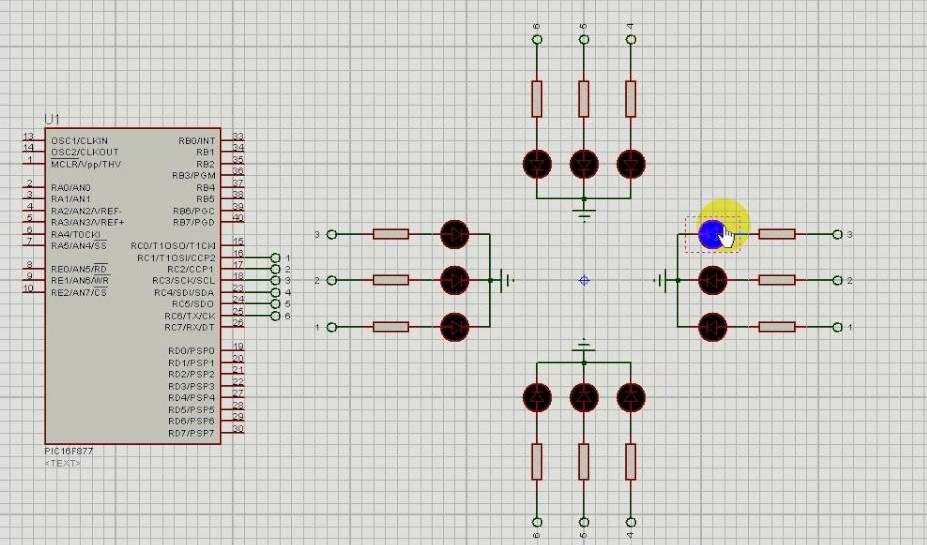
\includegraphics[width=5in]{source/picture/bai_1/pic2.jpg}
    \caption{\textit{Reference design for a 4 way traffic light}}
    \label{bai1_pic2}
\end{figure}

\subsection{Exercise 4}
Add \textbf{only one 7 led segment} to the schematic in Exercise 3. This component can be found in Proteus by the keyword \textbf{7SEG-COM-ANODE}. For this device, the common pin should be connected to the power supply and other pins are supposed to connected to PB0 to PB6. Therefore, to turn-on a segment in this 7SEG, the STM32 pin should be in logic 0 (0V).\\

Implement a function named \textbf{display7SEG(int num)}. The input for this function is from 0 to 9 and the outputs are listed as following:

\begin{figure}[!htp]
    \centering
    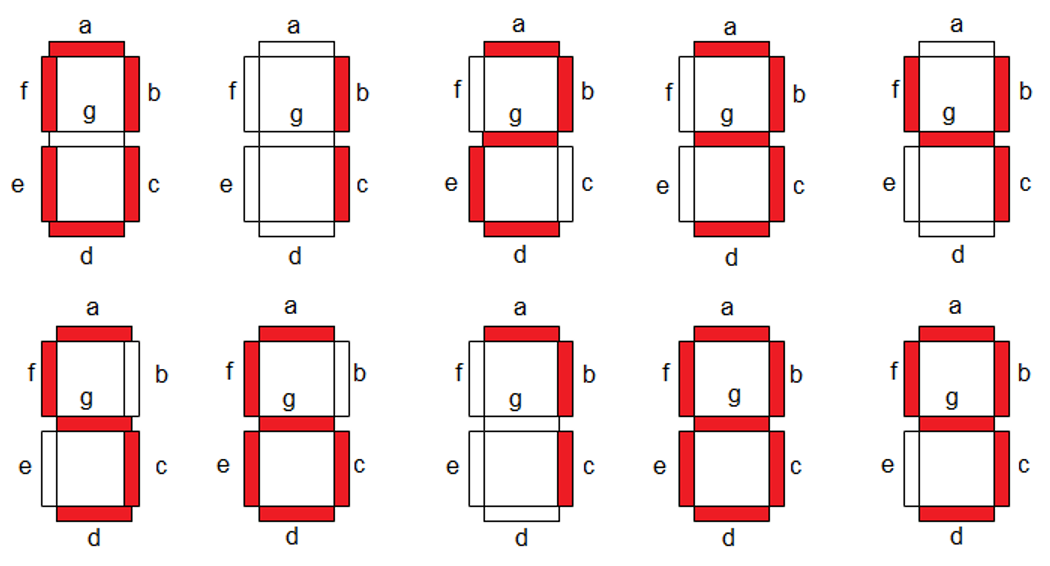
\includegraphics[width=4in]{source/picture/bai_1/pic3.PNG}
    \caption{\textit{Display a number on  7 segment LED}}
    \label{bai1_pic3}
\end{figure}

\newpage
This function is invoked in the while loop for testing as following:
\begin{lstlisting}[caption=An example for your source code]
int counter = 0;
while (1){
    if(counter >= 10) counter = 0;    
    display7SEG(counter++);
    HAL_Delay(1000);

}
\end{lstlisting}

\textbf{Report 1: } Present the schematic.\\

\begin{figure}[!htp]
    \centering
    \includegraphics[width=5in]{source/Image/bai4.png}
\end{figure}

\textbf{Report 2: } Present the source code for display7SEG function.
\begin{lstlisting}
void display7SEG(int num) {
	switch (num) {
		case 0:
			GPIOB->ODR = 0x0040; // 0100 0000
			break;
		case 1:
			GPIOB->ODR = 0x0079; // 0111 1001
			break;
		case 2:
			GPIOB->ODR = 0x0024; // 0010 0100
			break;
		case 3:
			GPIOB->ODR = 0x0030; // 0011 0000
			break;
		case 4:
			GPIOB->ODR = 0x0019; // 0001 1001
			break;
		case 5:
			GPIOB->ODR = 0x0012; // 0001 0010
			break;
		case 6:
			GPIOB->ODR = 0x0002; // 0000 0010
			break;
		case 7:
			GPIOB->ODR = 0x0078; // 0111 1000
			break;
		case 8:
			GPIOB->ODR = 0x0000; // 0000 0000
			break;
		case 9:
			GPIOB->ODR = 0x0010; // 0001 0000
			break;
		default:
			break;
	}
}
\end{lstlisting}

\subsection{Exercise 5}
Integrate the 7SEG-LED to the 4 way traffic light. In this case, the 7SEG-LED is used to display countdown value.\\

In this exercise, only source code is required to present. The function display7SEG in previous exercise can be re-used.
\begin{figure}[!htp]
    \centering
    \includegraphics[width=5in]{source/Image/bai5.png}
\end{figure}
\begin{lstlisting}
unsigned int buffer = 0x0000;
void display7SEG_One(int num) {
	buffer = buffer & 0xFF00;
	switch (num) {
		case 0:
			buffer += 0x0040; // 0100 0000
			break;
		case 1:
			buffer += 0x0079; // 0111 1001
			break;
		case 2:
			buffer += 0x0024; // 0010 0100
			break;
		case 3:
			buffer += 0x0030; // 0011 0000
			break;
		case 4:
			buffer += 0x0019; // 0001 1001
			break;
		case 5:
			buffer += 0x0012; // 0001 0010
			break;
		case 6:
			buffer += 0x0002; // 0000 0010
			break;
		case 7:
			buffer += 0x0078; // 0111 1000
			break;
		case 8:
			buffer += 0x0000; // 0000 0000
			break;
		case 9:
			buffer += 0x0010; // 0001 0000
			break;
		default:
			break;
	}
	GPIOB->ODR = buffer;
}
void display7SEG_Two(int num) {
	buffer = buffer & 0x00FF;
	switch (num) {
		case 0:
			buffer += 0x4000; // 0100 0000
			break;
		case 1:
			buffer += 0x7900; // 0111 1001
			break;
		case 2:
			buffer += 0x2400; // 0010 0100
			break;
		case 3:
			buffer += 0x3000; // 0011 0000
			break;
		case 4:
			buffer += 0x1900; // 0001 1001
			break;
		case 5:
			buffer += 0x1200; // 0001 0010
			break;
		case 6:
			buffer += 0x0200; // 0000 0010
			break;
		case 7:
			buffer += 0x7800; // 0111 1000
			break;
		case 8:
			buffer += 0x0000; // 0000 0000
			break;
		case 9:
			buffer += 0x1000; // 0001 0000
			break;
		default:
			break;
	}
	GPIOB->ODR = buffer;
}
  int counter = 10;
  int reset_counter = 10;
  int time_7SEG1 = 3, time_7SEG2 = 5;
  int flag1, flag2; // red = 0 yellow = 1 green = 2
  while (1)
  {
	  if (counter == 7) {
		  time_7SEG1 = 2;
	  } else if (counter == 5) {
		  time_7SEG1 = 5;
	  } else if (counter == 0) {
		  time_7SEG1 = 3;
	  }
	  if (counter == 5) {
		  time_7SEG2 = 3;
	  } else if (counter == 2) {
		  time_7SEG2 = 2;
	  } else if (counter == 0) {
		  time_7SEG2 = 5;
	  }
	  if (counter <= 0) {
		  counter = reset_counter;
	  }
	  if (counter > 5) {
		  flag1 = 0;
	  } else if (counter > 2) {
		  flag1 = 2;
	  } else {
		  flag1 = 1;
	  }
	  if (counter > 7) {
		  flag2 = 2;
	  } else if (counter > 5) {
		  flag2 = 1;
	  } else {
		  flag2 = 0;
	  }
	  if (flag1 == 0) {
		  HAL_GPIO_WritePin(GPIOA, GPIO_PIN_1, SET);
		  HAL_GPIO_WritePin(GPIOA, GPIO_PIN_2, RESET);
		  HAL_GPIO_WritePin(GPIOA, GPIO_PIN_3, RESET);
	  } else if (flag1 == 1) {
		  HAL_GPIO_WritePin(GPIOA, GPIO_PIN_1, RESET);
		  HAL_GPIO_WritePin(GPIOA, GPIO_PIN_2, SET);
		  HAL_GPIO_WritePin(GPIOA, GPIO_PIN_3, RESET);
	  } else if (flag1 == 2) {
		  HAL_GPIO_WritePin(GPIOA, GPIO_PIN_1, RESET);
		  HAL_GPIO_WritePin(GPIOA, GPIO_PIN_2, RESET);
		  HAL_GPIO_WritePin(GPIOA, GPIO_PIN_3, SET);
	  }
	  if (flag2 == 0) {
		  HAL_GPIO_WritePin(GPIOA, GPIO_PIN_4, SET);
		  HAL_GPIO_WritePin(GPIOA, GPIO_PIN_5, RESET);
		  HAL_GPIO_WritePin(GPIOA, GPIO_PIN_6, RESET);
	  } else if (flag2 == 1) {
		  HAL_GPIO_WritePin(GPIOA, GPIO_PIN_4, RESET);
		  HAL_GPIO_WritePin(GPIOA, GPIO_PIN_5, SET);
		  HAL_GPIO_WritePin(GPIOA, GPIO_PIN_6, RESET);
	  } else if (flag2 == 2) {
		  HAL_GPIO_WritePin(GPIOA, GPIO_PIN_4, RESET);
		  HAL_GPIO_WritePin(GPIOA, GPIO_PIN_5, RESET);
		  HAL_GPIO_WritePin(GPIOA, GPIO_PIN_6, SET);
	  }
	  display7SEG_One(time_7SEG1);
	  display7SEG_Two(time_7SEG2);
	  time_7SEG1--;
	  time_7SEG2--;
	  counter--;
	  HAL_Delay(1000);
    /* USER CODE END WHILE */

    /* USER CODE BEGIN 3 */
  }
\end{lstlisting}

\subsection{Exercise 6}
In this exercise, a new Proteus schematic is designed to simublate an analog clock, with 12 different number. The connections for 12 LEDs are supposed from PA4 to PA15 of the STM32. The arrangement of 12 LEDs is depicted as follows.

\begin{figure}[!htp]
    \centering
    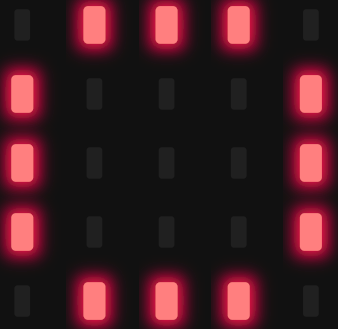
\includegraphics[width=3in]{source/picture/bai_1/pic4.PNG}
    \caption{\textit{12 LEDs for an analog clock}}
    \label{bai1_pic3}
\end{figure}

Report 1: Present the schematic.
\begin{figure}[!htp]
    \centering
    \includegraphics[width=5in]{source/Image/bai6.png}
\end{figure}
Report 2: Implement a simple program to test the connection of every single LED. This testing program should turn every LED in a sequence.
\begin{lstlisting}
  int counter = 12;
  int reset_counter = 12;
  unsigned int hex_num = 0x10;
  while (1)
  {
	  if (counter <= 0) {
		  counter = reset_counter;
		  hex_num = 0x10;
	  }
	  GPIOA->ODR = hex_num;
	  hex_num = hex_num << 1;
	  counter--;
	  HAL_Delay(1000);
    /* USER CODE END WHILE */

    /* USER CODE BEGIN 3 */
  }
\end{lstlisting}

\subsection{Exercise 7}
Implement a function named \textbf{clearAllClock()} to turn off all 12 LEDs. Present the source code of this function.

\begin{lstlisting}[caption=Function Implementation]
unsigned char status[12] = {};
void clearAllClock() {
	GPIOA->ODR = 0x0000;
	for (int i = 0; i < 11; i++) {
		status[i] = 0;
	}
}
\end{lstlisting}

\subsection{Exercise 8}
Implement a function named \textbf{setNumberOnClock(int num)}. The input for this function is from \textbf{0 to 11} and an appropriate LED is turn on. Present the source code of this function.
\begin{lstlisting}
unsigned char status[12] = {};
unsigned int buffer = 0x0000;
void setNumberOnClock(int num) {
	if (num < 0 || num > 11) {
		return;
	}
	if (status[num] == 0) {
		unsigned int hex_num = 0x10 << num;
		buffer += hex_num;
		status[num] = 1;
		GPIOA->ODR = buffer;
	}
}
\end{lstlisting}

\subsection{Exercise 9}
Implement a function named \textbf{clearNumberOnClock(int num)}. The input for this function is from \textbf{0 to 11} and an appropriate LED is turn off. 
\begin{lstlisting}
unsigned char status[12] = {};
unsigned int buffer = 0x0000;
void clearNumberOnClock(int num) {
	if (num < 0 || num > 11) {
		return;
	}
	if (status[num] == 1) {
		unsigned int hex_num = 0x10 << num;
		buffer -= hex_num;
		status[num] = 0;
		GPIOA->ODR = buffer;
	}
}
\end{lstlisting}

\subsection{Exercise 10}
Integrate the whole system and use 12 LEDs to display a clock. At a given time, there are only 3 LEDs are turn on for hour, minute and second information.
\begin{lstlisting}
unsigned char status[12] = {};
unsigned int buffer = 0x0000;
void clearAllClock() {
	GPIOA->ODR = 0x0000;
	buffer = 0x0000;
	for (int i = 0; i < 12; i++) {
		status[i] = 0;
	}
}
void setNumberOnClock(int num) {
	if (num < 0 || num > 11) {
		return;
	}
	if (status[num] == 0) {
		unsigned int hex_num = 0x10 << num;
		buffer += hex_num;
		status[num] = 1;
		GPIOA->ODR = buffer;
	}
}
void clearNumberOnClock(int num) {
	if (num < 0 || num > 11) {
		return;
	}
	if (status[num] == 1) {
		unsigned int hex_num = 0x10 << num;
		buffer -= hex_num;
		status[num] = 0;
		GPIOA->ODR = buffer;
	}
}
  GPIOA->ODR = 0x0000;
  unsigned char second = 0, minute = 0, hour = 0;
  while (1)
  {
	  second++;
	  if (second == 60) {
		  second = 0;
		  minute++;
	  }
	  if (minute == 60) {
		  minute = 0;
		  hour++;
	  }
	  if (hour == 12) {
		  hour = 0;
	  }
	  clearAllClock();
	  setNumberOnClock(second / 5);
	  setNumberOnClock(minute / 5);
	  setNumberOnClock(hour);
	  HAL_Delay(1000);
    /* USER CODE END WHILE */

    /* USER CODE BEGIN 3 */
  }
\end{lstlisting}